\documentclass[11pt]{article}
\usepackage{geometry}                % See geometry.pdf to learn the layout options. There are lots.
\geometry{letterpaper}                   % ... or a4paper or a5paper or ... 
%\geometry{landscape}                % Activate for for rotated page geometry
%\usepackage[parfill]{parskip}    % Activate to begin paragraphs with an empty line rather than an indent
\usepackage{graphicx}
\usepackage{amssymb}
\usepackage{epstopdf}
\usepackage{cite}
\usepackage{tipa}
\usepackage{subcaption}
\DeclareGraphicsRule{.tif}{png}{.png}{`convert #1 `dirname #1`/`basename #1 .tif`.png}





\title{Cross-Linguistic Neural Phoneme Embeddings for Computational Historical and Typological Linguistics}
\author{Marlon Betz}
%\date{}                                           % Activate to display a given date or no date

\begin{document}
\maketitle
\newpage
\tableofcontents

\section{Introduction}
Embeddings nowadays build the backbone of every Deep Learning NLP architecture. Due to their capacity to encode a vast amount of latent semantic and syntactic information without the need of previous manual construction, they gave rise to the contemporary Deep Learning boom, i.e. deep neural networks that can capture hidden features in data sets and by that have allowed for huge performance gains in numerous NLP fields. \\While embeddings are currently being used for several linguistic units such as characters\cite{kim2015character,dos2014learning,zhang2015character}, words \cite{mikolov2013efficient,mikolov2013distributed,pennington2014glove} or entire sentences \cite{kiros2015skip}, proper phonemes have been largely been excluded from this trend, although there are some data that would indeed allow for it and research areas where they could be of great use, especially in the fields of Computational Typological and Historical Linguistics, which the current deep learning boom has hardly touched yet. There, even though it is clear that some phonemes share more common features and such form natural classes, they are often treated as pure symbols that share a common distance between each other. Even phoneme representation models that do incorporate phonological features are often hand-crafted \cite{kondrak2000new,rama2016siamese} or include task-specific information that inherently suffer from restricted generalization abilities when used for other tasks \cite{jager2014phylogenetic}. Moreover, those methods usually reduce the number of possible phonemes to a minimum, getting rid of important information such as secondary or co-articulations. \\
In this paper, I will first a discuss a theoretical motivation for using data-driven phoneme embeddings instead of plain symbolic representations or hand-crafted feature encodings. I will then shortly take a look on the related research of character embeddings. A big part of this paper will then review several embedding models. I will then discuss intrinsic evaluation methods for the embeddings and use those to compare the performances of the previously described models. This is then followed by a discussion of several use cases that could be interesting for those interested in data-driven approaches to Typological and Historical Linguistics. Finally, I will recapitulate the benefits and drawbacks of phoneme embeddings in a final resume.
\section{Theoretical and Practical Motivation}
It is well-established that certain phonemes share phonological features, such as \textsc{[nasal]}, \textsc{[voice]} or \textsc{[labial]}. This implies that some phonemes are closer to each other than to other phonemes, given a certain distance measure incorporating such features. However, phonemes are nevertheless handled as pure symbols quite often, where the distance between phonemes does not vary. Even in the field of Historical Linguistics, where words are often given as phoneme sequences, symbolic string comparisons remain the backbone of most models. For instance, given the three hypothetical words /apa/, /aba/ and /aq"a/, purely symbolic string distances would estimate the distances between the words to be the same. However, /b/ and /p/ only differ in voice but are both labials, while /q"/ is an uvular ejective and hence should be less close to the labial phonemes.
It is indeed possible to incorporate such features by hand. However, this decision would either yield a tremendously tedious work if done for all phonemes to be worked with, or would be incomplete insofar as features that might be seen to be unnecessary for a certain task are left out and a big number of distinctive phonemes would merge. Moreover, such hand-crafted feature architectures do not directly allow for the conversion of one feature architecture into the other: A model designed for IPA cannot directly work with ASJP data and vice versa, as the symbols and their respective features are different for each model.
Embeddings can solve those problems: On the one hand, they allow for fine-grained distance measures between phonemes and thus overcome the symbolic constraint of equidistance. On the other hand, they are trained on data, which means all phonemes found in a corpus can be embedded in the embedding space without the need to create features by hand, given a corpus that is big enough to capture a variety of phoneme inventories to allow for unbiased phoneme comparisons beyond language boundaries.
Once having a reliable embedding space, it is further possible to use that space for other tasks without the need to train new task-specific embeddings. Embedding spaces in general allow for one-shot or zero-shot learning. This means that embeddings trained on some task can either be used for another task directly or by fitting a simple regression from one embedding space into the other, without the need to train new embeddings for a new task. This follows the idea that embeddings should incorporate as much information as possible, while for certain tasks some information might be irrelevant and can be left out.
\section{Related Research}
Word embeddings have proven to be a reliable tool for several NLP tasks. However, finer grained embedding models that take care of the internal structure of a word have been shown to give similar or even improved performance over traditional word embeddings as they are able to encode morphological \cite{dos2014learning} or semantic \cite{chen2015joint} information even for out-of-vocabulary items \cite{ling2015finding}. This follows the simple idea that since a word can be split up into its respective morphemes that encode morphosyntactic and semantic information, encoding subparts of a word instead of a the whole word should allow for better generalization for unseen words without the need to compute and store vector representations for every word type. 
\section{Embedding Models}
%\subsection{Count-based Embedding Models}
%\subsubsection{Latent Semantic Analysis}
%\subsubsection{GloVe}
%\subsubsection{SPPMI}
%\subsubsection{SPPMI-SVD}
\subsection{Neural Embedding Models}
\begin{figure}[t]
\centering
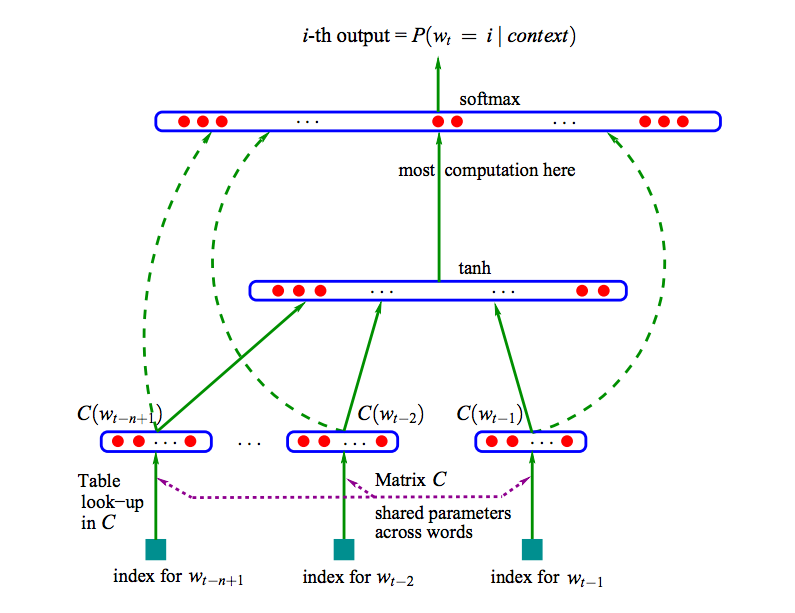
\includegraphics[width=0.75\textwidth]{bengio2006network}
\caption{The neural language model as proposed in \cite{bengio2003neural}.}
\label{fig:bengio2006network}
\end{figure}
Models that make use of  cooccurrence count matrix factorizations usually suffer from the need of storing huge amounts of data into working memory. Neural networks with hidden layers, on the other hand, have been proven to be able to approximate any given hidden function while they still allow for online or mini-batch training, which is a huge improvement over models that only work with whole data batches. Moreover they allow for fine-grained objective functions, where additional data can be introduced into the network to enhance the amount of information stored in the embeddings.
\subsubsection{Neural Language Models}
 \cite{bengio2003neural} pioneered as the first to introduce Neural Language Models in general. Here, a network with two hidden layers is proposed, where a first non-linear hidden layer with locally shared weights gives embeddings of single words in the given context window, while the next layer is a concatenation of the single word embeddings and another non-linear activation function and gives a context embedding. The last layer than is a softmax classifier that predicts the next word (cf. Figure \ref{fig:bengio2006network}). 
It later became clear that this model had two major drawbacks:
\begin{itemize}  
\item The softmax classifier needs to compute the probability of all word types in the vocabulary. This is a major flaw also of following models (see below).
\item The non-linear hidden layer severely worsened the convergence rate of the network.
\end{itemize}
\cite{collobert2008unified} then improved the model tremendously by getting rid of the expensive softmax classifier by introducing a score based loss function: 
\begin{equation}
J_{\theta} = \sum_{x\in X}\sum_{w\in V}\max(0,1-f_{\theta}(x)+f_{\theta}(x^{(w)}))
\label{eq:bengio2006network_loss}
\end{equation}
Here, the the correct windows x containing n words are sampled from the set of all possible windows X in the corpus, while for every window x, a corrupted version $x^{(w)}$ is produced by replacing the center word of $x$ by the another word of the vocabulary $V$. The objective then becomes maximizing the distance between the scores output by the model fore correct and the incorrect window with a margin of 1. The actual model then was still the same as in \cite{bengio2003neural}. This model could already embed semantically similar words close to each other, but still suffered from the non-linear hidden layer, which slowed down learning enormously (\cite{bengio2003neural} report a training time of 7 weeks for a vocabulary of 130000 word types)
\subsubsection{Word2Vec}
\begin{figure}[htbp] %  figure placement: here, top, bottom, or page
   \centering
   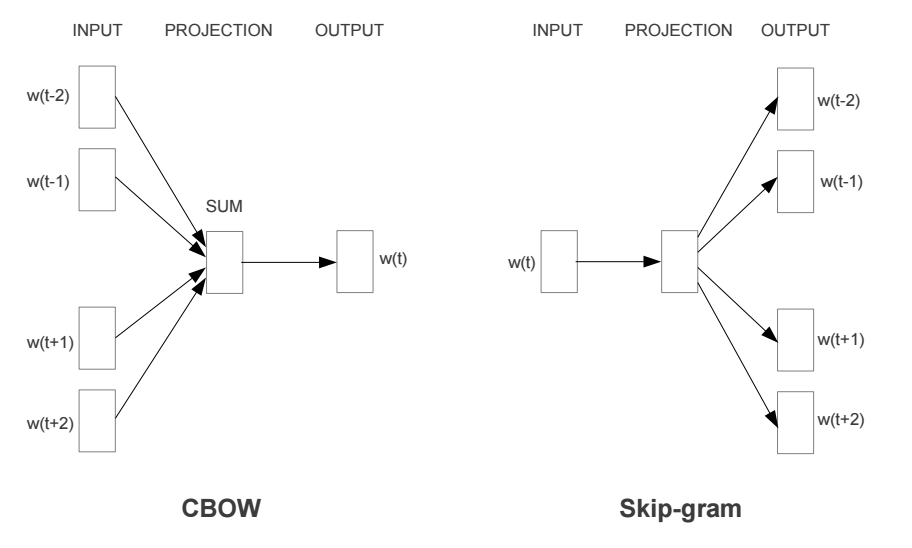
\includegraphics[width=0.75\textwidth]{word2vec} 
   \caption{The two common architectures of word2vec. The Continuous Bag-of-Words (CBOW) model predicts the current word based on the
context, and the Skip-gram predicts surrounding words given the current word. From \cite{mikolov2013efficient}.}
   \label{fig:word2vec}
\end{figure}
Among general-purpose embedding models in general and among neural embedding models in particular, the word2vec algorithm \cite{mikolov2013efficient,mikolov2013distributed} stands out as major breakthrough, as it offers good performance while the parameters to train are less then with the previous models. Different to the previous models in \cite{bengio2003neural,collobert2008unified}, which employ non-linear hidden layers, here the model only consists of a linear encoder layer that computes the actual embeddings. It can be seen as a full departure from traditional embedding models as a subgroup of language models towards a new kind of model family that in the first place tries to encode semantic and morphosyntactic information of a word rather than to predict the next word itself. Instead, the context window usually encompasses all surrounding words of a given target word instead of just the previous words. This makes it rather unhandy for true language modeling, but allows for much better incorporation of latent information. Moreover, the model can be trained in two ways: It either tries to predict the target word given its context (Continuous Bag-of-Words; CBOW) or tries to predict the context of a word given the target word itself (Skip-Gram, cf. Figure \ref{fig:word2vec}). The corresponding loss function for the CBOW model is given as 
\begin{equation}
J_{\theta} = \frac{1}{T} \sum_{t=1}^{T}\log p(w_{t}\mid w_{t-n},\dots,w_{t-1},w_{t+1},\dots,w_{t+n})
\label{eq:CBOW_loss}
\end{equation}

where $p(w_{t}\mid w_{t-1},\dots,w_{t-n+1})$ is given as a softmax

\begin{equation}
p(w_{t}\mid w_{t-1},\dots,w_{t-n+1}) = \frac{\exp(h^\top v'_{w_{t}}))}{\sum_{w_i \in V} \exp(h^\top v'_{w_i})} 
\label{eq:cbow_softmax_prob}
\end{equation}

while the loss for the Skip-Gram model is given as

\begin{equation}
J_{\theta} = \frac{1}{T} \sum_{t=1}^{T}\sum_{-n\leq j\leq n,\neq 0}\log p(w_{t+j}\mid w_{t})
\label{eq:skipgram_loss}
\end{equation}

where $p(w_{t+j}\mid w_{t})$ is again defined as a softmax
\begin{equation}
\log p(w_{t+j}\mid w_{t}) = \frac{\exp(v_{w_{t}}^\top v'_{w_{t+j}}))}{\sum_{w_i \in V} \exp(h^\top v'_{w_i})}
\label{eq:skipgram_softmax_prob}
\end{equation}
where $v_w_i$ is an input vector and $v'_w_i$ an output vector representation of a word $w_i$ and $h^\top$ the transpose of the sum of the output vectors of the words in the context. Again, the calculation of the softmax here includes summing over all contexts in the corpus, which computationally is expensive. Further research largely concentrated on finding a way to define $p$ as a memory- and time-friendly approximation of the true softmax probability. A first solution was given by using a hierarchical softmax classifier \cite{morin2005hierarchical} nstead. Here, the classifier layer is a binary tree with the actual words as leaves. At every node, the network learns to either follow the left or the right branch with a certain probability as in Eq. \ref{eq:skipgram_softmax_prob} that is equal to the sum of the child elements of the respective  branch, but is actually computed as the product of $h^\top$ and the output vector of the word at node $n$ pulled through a logistic sigmoid:

\begin{equation}
p(right|n,c) = \sigma(h^\top v'_n) 
\label{eq:hierarchicalsoftmax_nodeprob}
\end{equation}

This means  in order to calculate the softmax probability of word, we only have to follow the path down to the word leaf instead of summing over all vocabulary entries. For binary trees, this means we only have to pass at most $\log_2(\mid V\mid)$ nodes to calculate the probability of a word, which is a huge performance boost over the traditional softmax classifier. 


Another way of approximation the softmax is using Differentiated Softmax (cf.\cite{chen2015strategies}), where the idea is that rare words should help to adjust less parameters than  more frequent words. The fully connected softmax layer becomes a sparse matrix here, where certain blocks inside of that matrix are used to predict words with a certain frequency. \cite{chen2015strategies} mention their model is fast and accurate, but has less predictive power with rare words, as they are given less parameters to be predicted.



Another family of models approximate the true softmax via sampling. Here, it seems to be common to reformulate the softmax defintions from above. For instance, if we use negative log probabilities instead of raw probabilities and if we further use a more general score function $\mathcal{E}(w)$ instead of the more specific dot products of the context and word vectors and start with Eq.  \ref{eq:cbow_softmax_prob}, the loss function $J_{\theta}$ becomes 



\begin{equation}
J_\theta =\mathcal{E}(w) + \log \sum_{w_i \in V} \exp (-\mathcal{E}(w_i))
\label{eq:negative_reinforcement_1}
\end{equation}

For back-propagating the error, we calculate the gradients of this term:

\begin{equation}
\nabla_\theta J_\theta =\nabla_\theta \mathcal{E}(w) + \nabla_\theta \log \sum_{w_i \in V} \exp (-\mathcal{E}(w_i))
\label{eq:negative_reinforcement_2}
\end{equation}

\begin{equation}
\nabla_\theta J_\theta =\nabla_\theta \mathcal{E}(w) +\frac{1}{\sum_{w_i \in V} \exp (-\mathcal{E}(w_i))} \nabla_\theta  \sum_{w_i \in V} \exp (-\mathcal{E}(w_i))
\label{eq:negative_reinforcement_3}
\end{equation}


\begin{equation}
\nabla_\theta J_\theta =\nabla_\theta \mathcal{E}(w) +\frac{1}{\sum_{w_i \in V} \exp (-\mathcal{E}(w_i))}  \sum_{w_i \in V}\nabla_\theta \exp (-\mathcal{E}(w_i))
\label{eq:negative_reinforcement_4}
\end{equation}



\begin{equation}
\nabla_\theta J_\theta =\nabla_\theta \mathcal{E}(w) +\frac{1}{\sum_{w_i \in V} \exp (-\mathcal{E}(w_i))}  \sum_{w_i \in V} \exp (-\mathcal{E}(w_i))\nabla_\theta (-\mathcal{E}(w_i))
\label{eq:negative_reinforcement_5}
\end{equation}

which can be rewritten as 
\begin{equation}
\nabla_\theta J_\theta =\nabla_\theta \mathcal{E}(w) 
+\sum_{w_i \in V}  \frac{\exp (-\mathcal{E}(w_i))}{\sum_{w_i \in V} \exp (-\mathcal{E}(w_i))}  \nabla_\theta (-\mathcal{E}(w_i))
\label{eq:negative_reinforcement_6}
\end{equation}

Here, we can replace the softmax in the second term by $P(w_i)$ and reposition the negative coefficient:

\begin{equation}
\nabla_\theta J_\theta =\nabla_\theta \mathcal{E}(w) 
-\sum_{w_i \in V}  P(w_i)  \nabla_\theta (\mathcal{E}(w_i))\label{eq:negative_reinforcement_7}
\end{equation}

As one can see, we basically end up with a positive and a negative reinforcement term. As the negative reinforcement term is basically the gradient of $\mathbb{E}_{w_i\sim P}$, the final reformulation of the softmax is then given as in Eq. \ref{eq:final_negative_reinforcement}.
\begin{equation}
\nabla_\theta J_\theta =\nabla_\theta \mathcal{E}(w)  - \mathbb{E}_{w_i\sim P}[\nabla _{\theta}\mathcal{E}(w_i)] 
\label{eq:final_negative_reinforcement}
\end{equation}

The goal of sampling-based approaches is now to approximate the negative reinforcement term $\mathbb{E}_{w_i\sim P}[\nabla _{\theta}\mathcal{E}(w_i)] $ without going over the whole vocabulary.
Earlier models used some forms of Importance Sampling \cite{liu2008monte,bengio2003quick,bengio2008adaptive,cho2015using}, where a proposal distribution $Q$ is used to approximate $P$. Although Importance sampling seems to provide a speed-up over the standard softmax, the model suffers from divergence issues.
Another group of sampling models does not try to estimate the probability of a word directly but uses an auxiliary loss that as a by-product produces probability estimates of correct words. Noise Contrastive Estimation (NCE, \cite{gutmann2010noise,mnih2012fast}) trains a model to differentiate between a true word $w_i$ and noise data $\tilde{w}_{ik}$, where $k$ is the number of noisy data points. As a start point, one can use a logistic regression loss that minimized the negative log-likelihood as in Eq \ref{eq:nce_1}, where $Q$ is a noise distribution:

\begin{equation}
J_{\theta}  = - \sum_{w_i \in V} [\log P(y=1|w_i,c_i) + k \mathbb{E}_{\tilde{w}_{ik}\sim Q}[\log P (y = 0|\tilde{w}_{ik},c_i)]]
\label{eq:nce_1}
\end{equation}

Since we want to avoid summing over all words in the vocabulary to estimate $ \mathbb{E}_{\tilde{w}_{ik}\sim Q}$, we substitute it with the mean as a Monte Carlo estimate, which leaves us with the sum over all log probabilities of the $k$ noisy words:

\begin{equation}
J_{\theta}  = - \sum_{w_i \in V} [\log P(y=1|w_i,c_i) + \sum_{j=1}^{k}\log P (y = 0|\tilde{w}_{ik},c_i)]
\label{eq:nce_2}
\end{equation}

As $w_i$ is sampled from the true Distribution $P$ while $\tilde{w}_{ik}$ comes from the noise distribution $Q$, this leaves us with a mixture model, where the probability of sampling a specific word with the corresponding label (that is, whether it comes from the true distribution in the training set or is noise) can be given as 

\begin{equation}
P(y,w|c) = \frac{1}{k+1}P(w|c)+\frac{k}{k+1}Q(w)\label{eq:nce_3}
\end{equation}

This can then be used to estimate the probability of the word to come from the true distribution:

\begin{equation}
P(y=1|w,c) = \frac{\frac{1}{k+1}P(w|c)}{\frac{1}{k+1}P(w|c)+\frac{k}{k+1}Q(w)}
\label{eq:nce_4}
\end{equation}

which can be simplified to
\begin{equation}
P(y=1|w,c) = \frac{P(w|c)}{kP(w|c)+Q(w)}
\label{eq:nce_5}
\end{equation}

Here, instead of taking the traditional softmax for  $P(w|c)$, NCE allows for a reparametrization of it: instead of summing over all probabilities in the lexicon to normalize the data, the denominator of the softmax is substituted by a parameter $Z(c)$ that is estimated by the model itself. In fact, and report equal performance while setting $Z(c)$ to 1, that is, the model learns to normalize the probabilities completely on its own. Coming from the definition of this probability in the CBOW architecture from Eq. \ref{eq:cbow_softmax_prob}, this leaves us with the probability of a word given a context as 

\begin{equation}
P(w|c) = \exp (h^{\top}v'_w)
\label{eq:nce_6}
\end{equation}

Inserting this into Eq. \ref{eq:nce_5}, we have

\begin{equation}
P(y=1|w,c) = \frac{\exp(h^{\top}v'_w)}{\exp(h^{\top}v'_w)+kQ(w)}
\label{eq:nce_6}
\end{equation}

which can be inserted into the logistic loss from  Eq. \ref{eq:nce_2} to yield the final NCE loss:


\begin{equation}
J_{\theta}  = - \sum_{w_i \in V} [\log  \frac{\exp(h^{\top}v'_{w_{i}})}{\exp(h^{\top}v'_{w_{i}})+kQ(w_i)} + \sum_{j=1}^{k}\log (1- \frac{\exp(h^{\top}v'_{\tilde{w}_{ij}})}{\exp(h^{\top}v'_{\tilde{w}_{ij}})+kQ({\tilde{w}_{ij}})})]
\label{eq:nce_7}
\end{equation}

The probably most prominent sampling model, however, is the Negative Sampling Model (NEG). Building on NCE, it diverges from it insofar as it naively assumes that $kQ(w)=1$. This yields Eq. \ref{eq:nce_6} as 

\begin{equation}
P(y=1|w,c) = \frac{\exp(h^{\top}v'_w)}{\exp(h^{\top}v'_w)+1}
\label{eq:neg_sampling_1}
\end{equation}

which is equal to the NCE loss as long as $k = |V|$ and Q is uniform. Eq. \ref{eq:neg_sampling_1} can then be reformulated as a logistic sigmoid:
\begin{equation}
P(y=1|w,c) = \frac{1}{1+\exp(-h^{\top}v'_w)}
\label{eq:neg_sampling_2}
\end{equation}

Inserted into the logistic regression loss, this yields
\begin{equation}
J_{\theta}  = - \sum_{w_i \in V} [\log \frac{1}{1+\exp(-h^{\top}v'_w)} 
+ \sum_{j=1}^{k}\log (1- \frac{1}{1+\exp(-h^{\top}v'_{\tilde{w}_{ij}})})]
\label{eq:neg_sampling_3}
\end{equation}

By simplification and substitution of the sigmoid term with $\sigma = \frac{1}{1+\exp(-x)}$, this derives the NEG loss:
\begin{equation}
J_{\theta}  = - \sum_{w_i \in V} [\log \sigma(h^{\top}v'_w)
+ \sum_{j=1}^{k}\log \sigma(-h^{\top}v'_{\tilde{w}_{ij}})]
\label{eq:neg_sampling_3}
\end{equation}

For a more in-depth analysis of NEG, see \cite{goldberg2014word2vec}.
\\\\As NEG is only equivalent to NCE when $k = |V|$ holds and $Q$ is uniform, this has a large impact on the performance of NEG when when used as a proper language model. As it cannot approximate the true softmax in practice, it gives poor performance on typical intrinsic language model evaluation tasks such as perplexity estimation, while it shows superior performance on embedding-specific evaluations such as similarity measures.


\begin{figure}[htbp] %  figure placement: here, top, bottom, or page
   \centering
   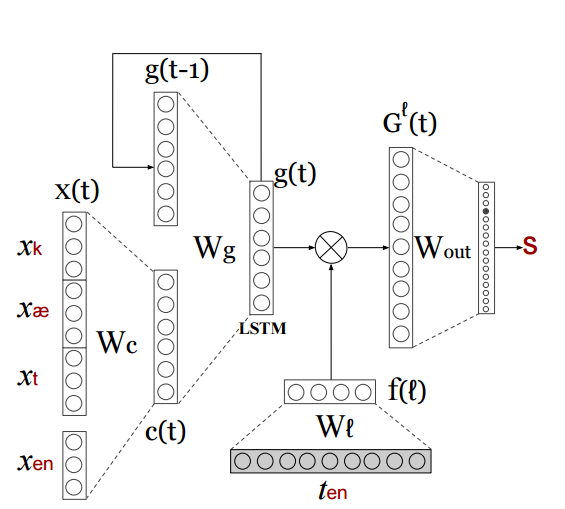
\includegraphics[width=0.75\textwidth]{polyglotLM} 
   \caption{The Polyglot Language Model. From \cite{tsvetkov2016polyglot}}
   \label{fig:plm}
\end{figure}


\subsubsection{Polyglot Neural Language Models}

One of the reasons why word2vec has become the most popular neural embedding model (and probably the most popular embedding model in general) is that it does not involve any hidden layers that would affect the training speed performance. However, with the rise of Long Short-term Memory Networks (LSTM, \cite{hochreiter1997long}), there is an increase of research on embeddings trained jointly with LSTMs to predict tokens or whole sequences \cite{chen2015joint,ling2015finding,kim2015character,dos2014learning}, while some learn them jointly with convolutional models \cite{zhang2015character}. One family of models important for our case are Polyglot Neural Language Models (PLM) \cite{tsvetkov2016polyglot}. Here, a deep model tries to predict the next phoneme given the previous phonemes, the language of the whole sequence as well as typological information from WALS \cite{wals}, PHOIBLE \cite{phoible} and Ethnologue \cite{lewis2015ethnologue} (see Fig. \ref{fig:plm}). 
The model first embeds the whole context into a hidden local context representation $c_t$

\begin{equation}
c_t = W_{x_{x}}x_t + W_{c_{lang}}x_{lang}+b_c
\label{eq:plm_1}
\end{equation}
where $x_t$ is a character embedding for character $c_t$ at position $t$, $x_{lang}$ is a one-hot vector for the respective language of the sequence and $b_c$ a bias for the character $c$. This then is fed into an LSTM to yield a global context layer $g_t$

\begin{equation}
g_t = LSTM(c_t,g_{t-1}) 
\label{eq:plm_2}
\end{equation}

Typological language information (such as if a single segment is represented in the phoneme inventory of a given language, or if there is a minimal contrast between the segment and another one in the phoneme inventory) is first mapped into a low-dimensional space to obtain a dense representation $f_\ell$

\begin{equation}
f_\ell = \tan(W_\ell t_\ell + b_\ell) 
\label{eq:plm_3}
\end{equation}


and then multiplied with the global context vector using Hadamard multiplication, yielding a gloval context-language matrix $G_t^\ell$
\begin{equation}
G_t^\ell = g_t \otimes f_\ell^\top 
\label{eq:plm_4}
\end{equation}


The resulting matrix is then vectorized into a column vector and an output sequence is computed:

\begin{equation}
p(\phi_t = i | \phi_i,\ldots,\phi_{t-1},\ell) = softmax(W_{out}vec(G_t^\ell)+b_{out})_i 
\label{eq:plm_5}
\end{equation}

Accordingly, the loss function here is a categorical cross-entropy $H(\phi,\hat{\phi})$ over all phonemes:

\begin{equation}
H(\phi,\hat{\phi}) = - \sum_i \hat{\phi}_i \log \phi_i
\label{eq:plm_6}
\end{equation}

The authors report superior perplexity over a baseline LSTM model, even with the typological information left out. Also downstream experiments on loan word detection and  speech synthesis leave the PLM model superior over the baseline LSTM model.

\section{Evaluation}
\subsection{Data}
For this paper, the data provided by the Automatic Similarity Judgement Program (ASJP,) will serve as a training corpus. ASJP provides wordlists of roughly 7200 languages, where each word is given as a string of phonemes. This vast amount of different phoneme inventories will allow for the unbiased comparison of phonemes over language boundaries. However, ASJP does not make use of IPA, but a simplified phonemic alphabet that is based on ASCII-characters. This makes it possible to incorporate data where no detailed IPA description is given, but might also reduce the quality of the resulting embedding space, as latent features that might be encoded in more specific IPA descriptions are merged. An overview of the ASJP phonemes and their IPA counterparts are given in the appendix.
\subsection{Intrinsic Evaluation}
\label{Intrinsic Evaluation}

Embeddings are commonly evaluated using \textit{intrinsic} and \textit{extrinsic} tests.
Intrinsic evaluation methods allow for the direct comparison of different models of embedding algorithms. Here the underlying assumption is that the embedding space itself should encode certain information. For word embeddings, this usually accumulates in relatedness, analogy, categorization or selectional preference tests \cite{schnabel2015evaluation}. They all have in common that the predicted outcome given a certain model is compared to a gold standard. The problem in our case is that for phoneme embeddings, there is hardly any pre-defined gold standard available, especially not for ASJP data. For this reason I will restrict the intrinsic evaluation part to analogy tests of the sort of those made popular by \cite{mikolov2013distributed}. I hand-crafted an analogy table of 108 analogy tasks where each line is of the form 

\begin{equation}
v(phoneme_1) + v(phoneme_2) -  v(phoneme_3) \approx v(phoneme_4)
\end{equation}

where $v(phoneme_1)$ is the vector corresponding to $phoneme_1$ and $v(phoneme_2) - v(phoneme_3)$ can be seen as the latent phonological information available in $phoneme_2$ but not in $phoneme_3$,  while $v(phoneme_1) + v(phoneme_2) -  v(phoneme_3) $ is then this latent phonological information added to $phoneme_1$, which should be close to the vector corresponding to $phoneme_4$. For example, in

\begin{equation}
v(\textbf{/i/} ) + v(\textbf{/u*/} ) -  v(\textbf{/u/} ) \approx v(\textbf{/i*/} )
\end{equation}
$v(\textbf{/u*/} ) -  v(\textbf{/u/} )$ describes a latent feature that should correspond to \textsc{[+nasalized]}, which is then added to the phoneme \textbf{/i/} to yield a nasalized \textbf{/i*/}. The latent features should correspond to accepted phonological distinctive features such as \textsc{[voice]}, \textsc{[labial]} or \textsc{[aspirated]}. For this task it is important that the target phoneme should only differ in one phonological feature from the source phoneme to allow for a detailed evaluation of the generalization abilities of the model in the latent feature space. Most tests concentrate on plosives and vowels, as they should appear most frequently in the data. The full list of analogy tasks can be found in the appendix. Here, accuracy serves as a test metric as the target phoneme embedding should be the at most $n$ -closest embedding to the predicted point in the embedding space. The parameter $n$ here serves as a threshold to allow for the fact that a prediction should still be good if the target phoneme is at least close to the predicted phoneme.
To compare the performance of the different embedding models, an extensive grid search over several hyperparameters was performed:
\begin{itemize}
\item Model architecture: CBOW, Skip-gram
\item Classifier: Softmax, negative sampling
\item Embedding dimensions: $[2, 5,10, 20, 50, 100, 150, 200, 400 ]$
\item Context window size: $[1,2,3,4,5,8]$
\item Number of negative samples: $[1, ..., 21]$
\end{itemize}
An analogy task is thought to be  For each hyperparameter setting, an ensemble of three models was trained simultaneously. Each model iterated five times over the corpus, which consists of all words from the ASJP corpus given the language they belong to is neither artificial nor reconstructed. Every word is moreover bracketed by word boundary tokens.

\begin{figure}[h] %  figure placement: here, top, bottom, or page
   \centering
   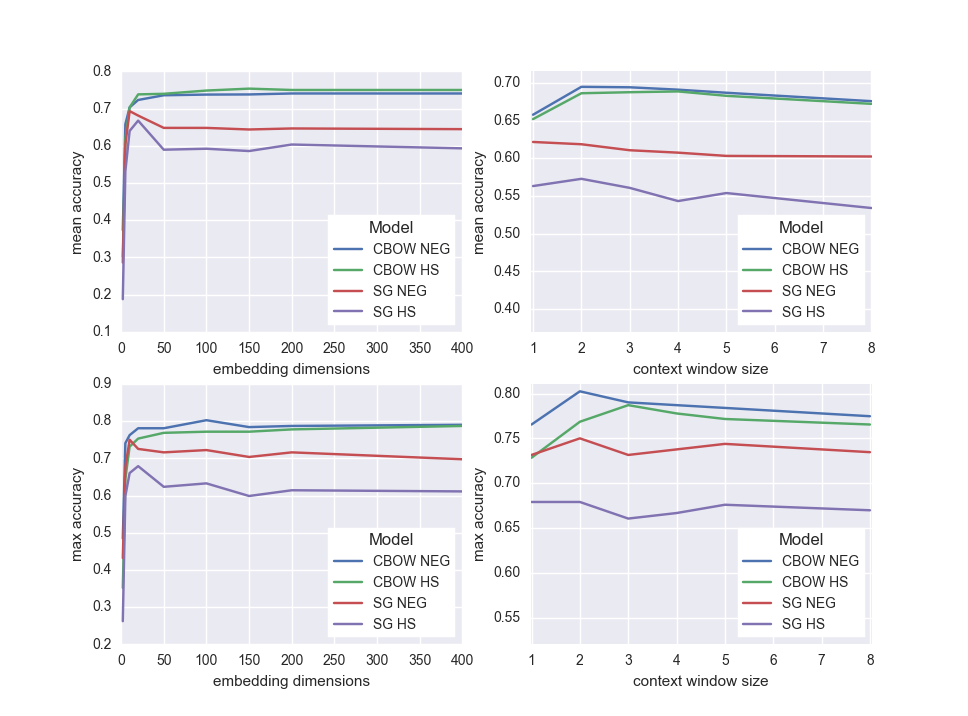
\includegraphics[width=\textwidth]{4models_comparison_meanMax} 
   \caption{Mean (top) and maximal (bottom) accuracy of the for models evaluated with regard to the number of embedding dimensions (left) and context window size (right) over all other hyperparameters.}
   \label{fig:4models_comparison}
\end{figure}


\begin{figure}[h] %  figure placement: here, top, bottom, or page
   \centering
   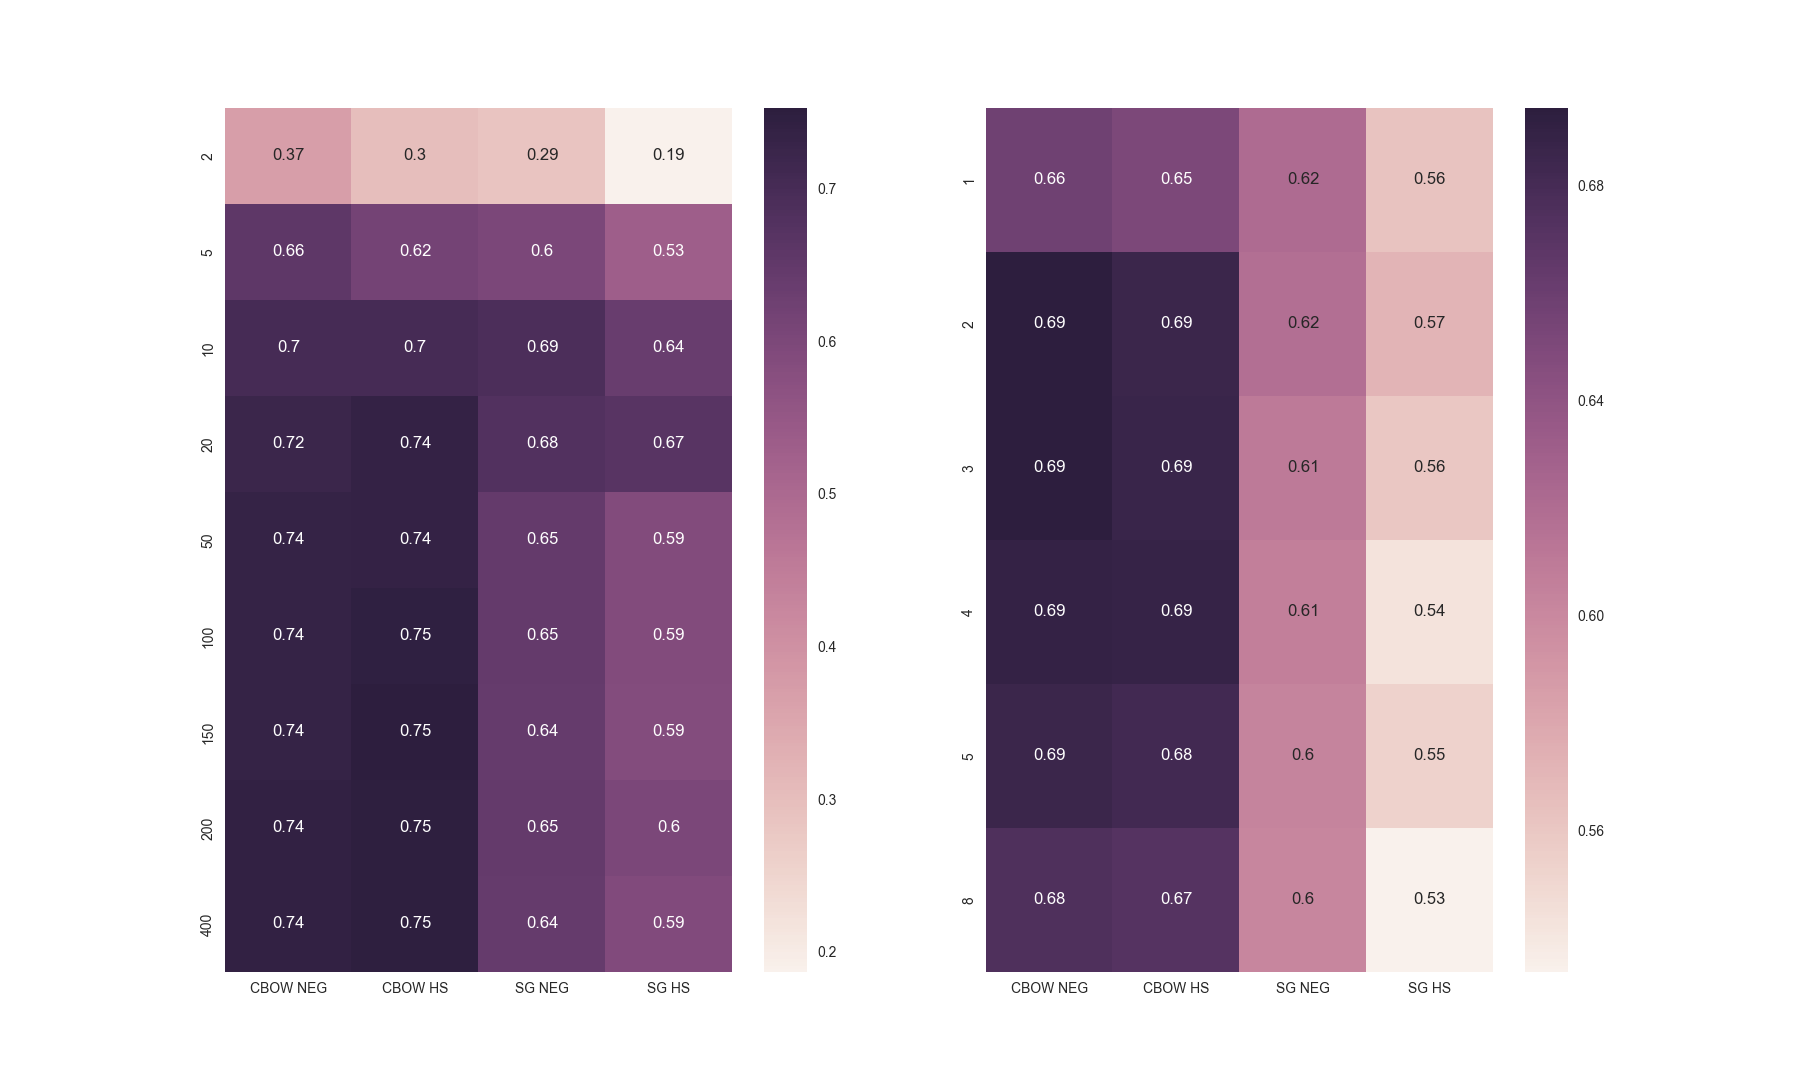
\includegraphics[width=\textwidth]{4models_comparison_meanValues} 
   \caption{Mean accuracies of the four models tested, over the number of embedding dimensions (left) and the context window size (right)}
   \label{fig:4models_comparison_meanValues}
\end{figure}


\begin{figure}[h] %  figure placement: here, top, bottom, or page
   \centering
   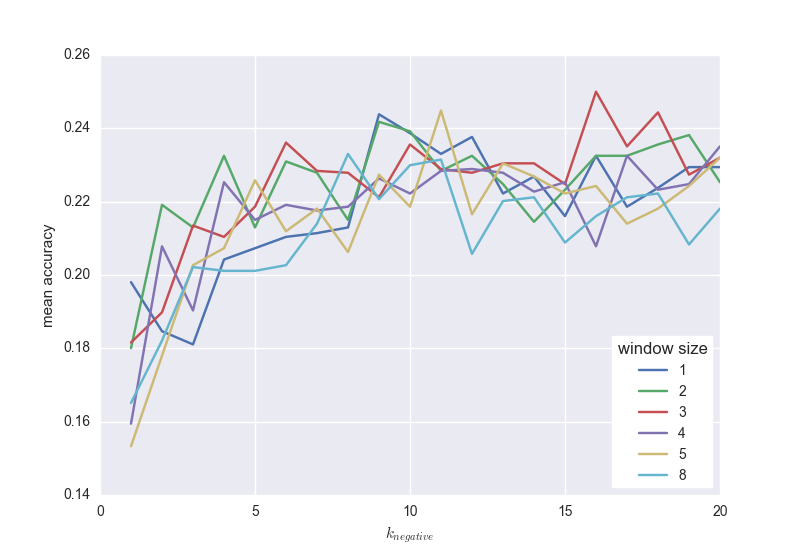
\includegraphics[width=0.8\textwidth]{acc_k_neg_vs_windowSize} 
   \caption{Mean and maximal accuracies of the skip-gram model with regard to the window size and number of negative samples over all other parameters.}
   \label{fig:acc_k_neg_vs_windowSize}
\end{figure}

\begin{figure}[h] %  figure placement: here, top, bottom, or page
   \centering
   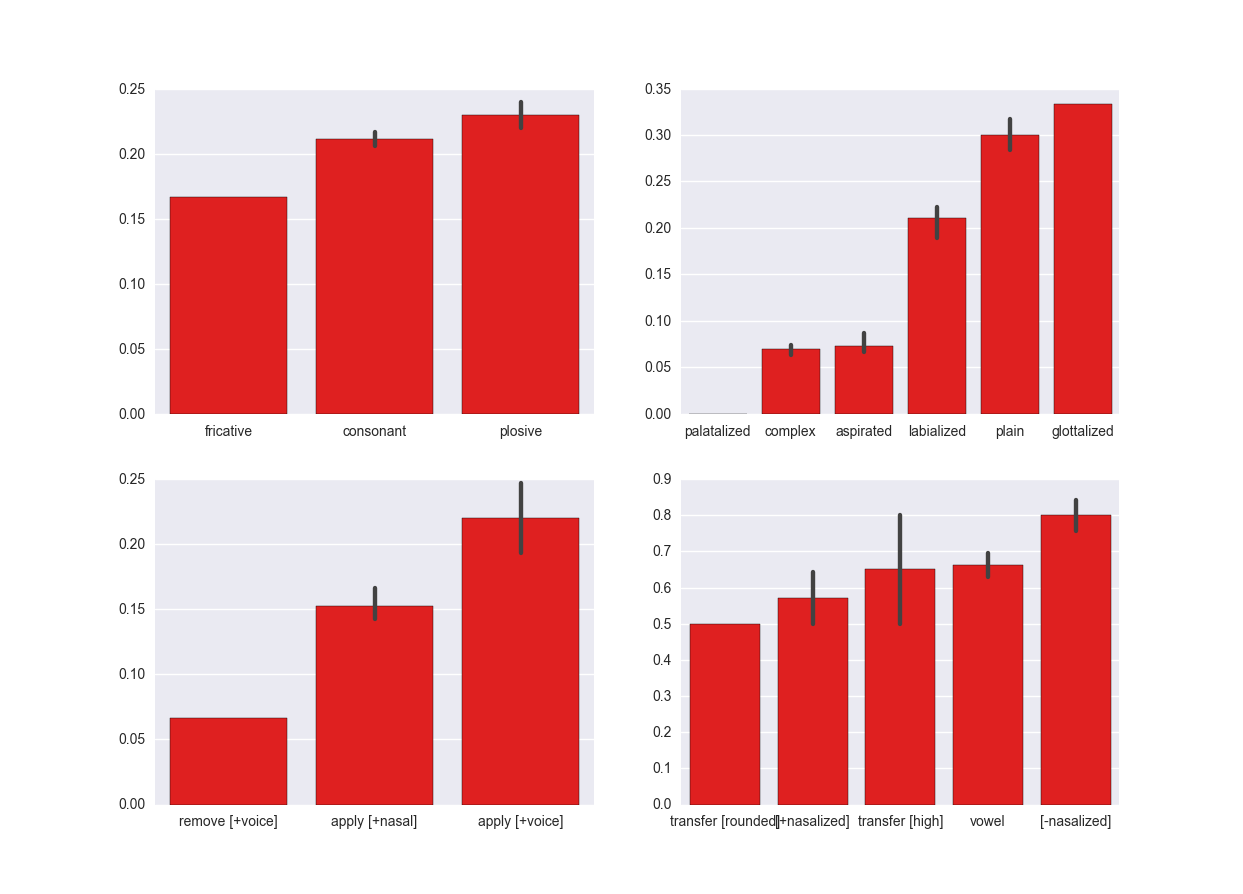
\includegraphics[width=\textwidth]{detailed_evaluation_topn1} 
   \caption{Mean accuracies for analogies with an analogy threshold of 1. The baseline model does not seem to be able to capture the compositionality of the latent features too well. (top left) Accuracy is best for plosives across plain pulmonic as well as more complex articulations, while fricatives perform much worse. (top right) Plain pulmonic consonant phonemes yield acceptable performance, while glottalized phonemes at least yield reasonable results. Among complex articulations, which all perform disasterously,  labialized phonemes yield best results, while aspirated and palatalized phonemes perform even worse. (bottom left) Adding voice works better than removing it or adding nasality. (bottom right) Vowel analogies work far better than consonant analogies. This should be due to the small number of possible vowel phonemes.}
   \label{fig:detailed_evaluation_consonants_topn1}
\end{figure}

\begin{figure}[h] %  figure placement: here, top, bottom, or page
   \centering
   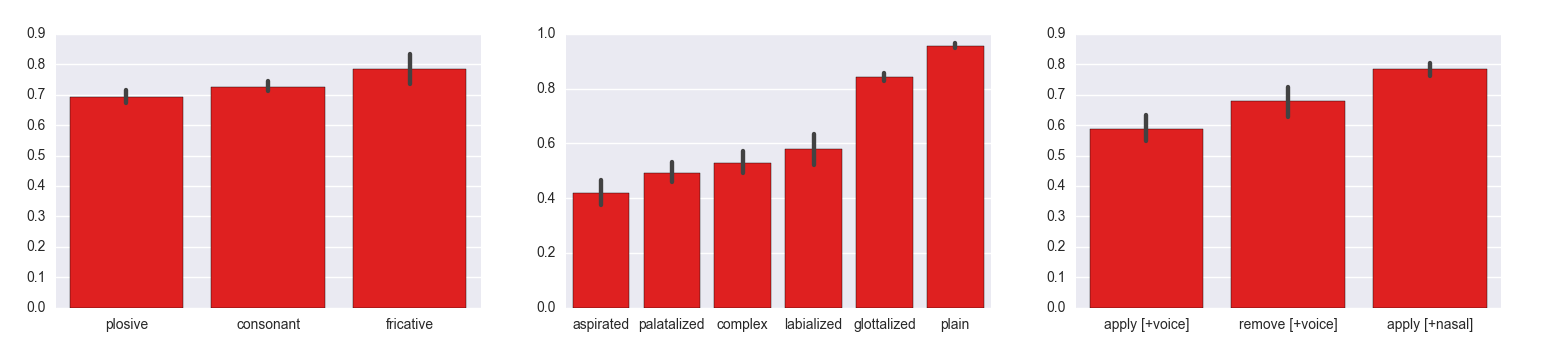
\includegraphics[width=\textwidth]{detailed_evaluation_topn20} 
   \caption{Mean accuracies for consonant analogies with an analogy threshold of 20. Here, the model is expected to yield better results, as wrong predictions are not as penalizing. (left) Accuracy is reasonable for plosives across plain pulmonic as well as more complex articulations. For fricatives, the accuracy is higher, but fricatives were only evaluated for plain pulmonic articulation. (middle) Plain pulmonic consonant phonemes nearly yield optimal accuracy, while glottalized phonemes still yield good results. Among complex articulations,  labialized phonemes yield best results, while aspirated and palatalized phonemes perform far under average. (right) Removing voice yields better results than adding it.  Applying nasality to plosives even performs better.}
   \label{fig:detailed_evaluation_consonants}
\end{figure}

\begin{figure}[h] %  figure placement: here, top, bottom, or page
   \centering
   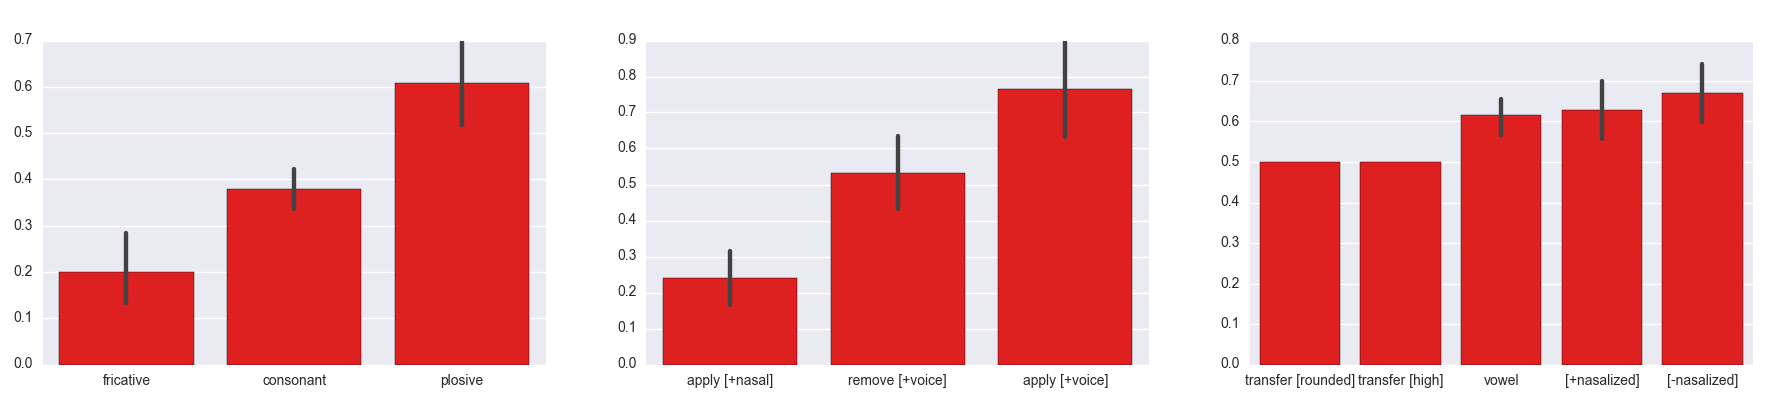
\includegraphics[width=\textwidth]{detailed_evaluation_topn1_poooled} 
   \caption{Mean accuracies for analogies with an analogy threshold of 1 on the pooled consonant phonemes. Here, the model is also expected to yield better results, the number of latent features should be reduced. (left) Accuracy is doubled compared with the unpooled phonemes. (middle) Adding voice works quite well, while removing it still yields acceptable performance. Applying nasality again works quite bad. (right) Vowel analogy tasks seem to work reasonably well.}
   \label{fig:detailed_evaluation_topn1_poooled}
\end{figure}

\begin{figure}[h] %  figure placement: here, top, bottom, or page
   \centering
   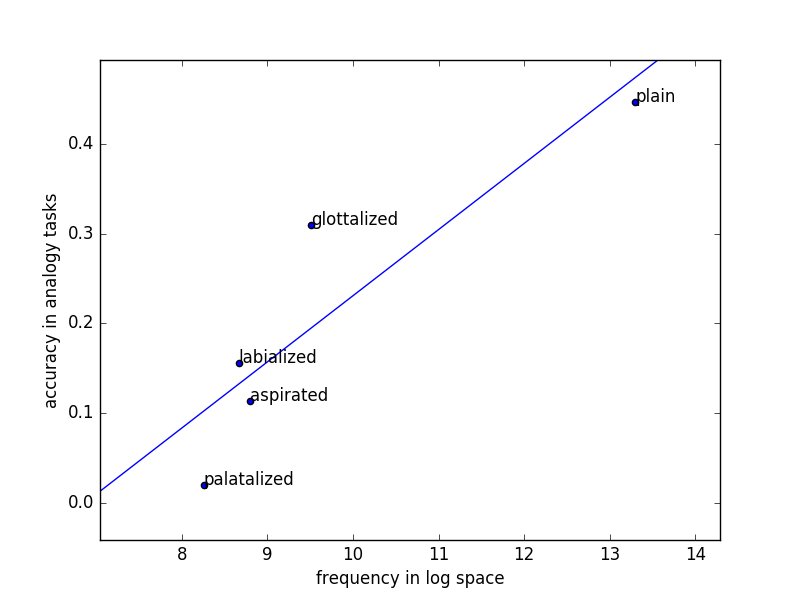
\includegraphics[width=0.5\textwidth]{freq_acc_correlation_logspace_topn1} 
   \caption{Frequency plotted against mean accuracy in log space. It is clearly visible how the bad performance of the complex phonemes is due to their underrepresentation in the corpus.}
   \label{fig:freq_acc_correlation_logspace}
\end{figure}



Figure \ref{fig:4models_comparison} and \ref{4models_comparison_meanValues} shows how CBOW clearly yields better results than skip-gram once the number of embedding dimensions increases. Hierarchical softmax further outperforms negative sampling with regard to mean accuracy slightly in the case of CBOW and severely in the case of Skip-gram. It can further be seen that 50 dimensions might already be enough for good accuracy and that more dimensions might even decrease performance at least for the negative sampling model, while a context window of 2 phonemes seems to maximize accuracy for all models.. Figure \ref{fig:acc_k_neg_vs_windowSize} further suggests that for negative sampling, the performance should not change too much with more than 10 negative samples.

The poor results with an analogy threshold $n = 1$  might suggest that the model is weak. However, in order to check if the model at least learns to cluster related phonemes together, another grid search was performed with an analogy threshold $n = 20$ that allows for less accurate predictions still to be valid. The model indeed seems to learn to capture latent phonological features, even though the compositional quality of the learned features seems far from perfect and shows big variance. 

For a more detailed evaluation, an ensemble of 10 models (CBOW with hierarchical softmax, 100 embedding dimensions, context window of 2 phonemes) was trained on the corpus (Figure \ref{fig:detailed_evaluation_consonants}). Analogy tasks with a threshold of 1 yield reasonable results for vowels, while for consonants the model's accuracy is far worse. The performance for complex phonemes is even worse. This might be connected to an underrepresentation of those complex phonemes in the corpus, which does not let the model generalize well.
In fact, the quality of the phoneme embeddings is correlated with their frequency in the corpus (Pearson correlation 0.9, Spearman correlation 0.9, Figure \ref{freq_acc_correlation_logspace_topn1}). This leads to the question if one should not indeed follow the example of others \cite{rama2016siamese,jager2014phylogenetic} and pool coarticulations and non-pulmonic phonemes with the plain pulmonic ones to allow for at least reasonable analogy performance over the whole corpus. 

\subsection{Phonemic String Comparison}
An often found sub-task in Computational Historical Linguistics are string comparisons. For instance, when trying find cognates, the basic assumption is that words that are etymologically related should show similar phonemic shape. The standard way here is using symbolic string distances such as the normalized Levenshtein distance. However, this assumes that phonemes are equidistant to each other. Weighted string comparisons, either hand-crafted of learned, try to account for the fact that some phonemes are closer to each other than to others. 
Using embeddings for string comparison means that one has to embed the sequence of phoneme embeddings of all words to be compared into some common latent space. Such word embeddings would then be close to each other if the words share similar phonological information and hence would inherently allow for weighted comparisons. 
\subsection{Modeling Sound Change}
\subsection{Proto-Form Reconstruction}
Especially for graphic data, the benefits of generative models, especially generative auto-encoders, lead to rising interest in such models. Here, a latent variable is used to approximate the expected output of a network. A quite simplistic model of sound change would be that the proto-form should contain information common to all daughter words, that is, the proto-form should be some sort of mean of all daughter words. If we now train such a model to encode and decode words and further cluster all words belonging to a certain cognate class, the centroid of such clusters should correspond to the underlying proto-form of the given words.
\subsection{Phoneme Inventory Clustering}
\section{Resume}

\bibliographystyle{apa}
\bibliography{references} 
\section{Appendix}
\begin{table}[h]
\centering
\tiny
\caption{Consonant analogy tests. All analogy tasks consist of 2 positive values, one negative value and a target value, as described in \ref{Intrinsic Evaluation}.}
\begin{tabular}{ l | l | l }
\hline \multicolumn{3}{l}{voiceless plosive $\rightarrow$ nasal via unvoiced plosive}\\  \hline
positive & negative & target \\ \hline
p, n & t & m \\
t, m & p & n \\
k, n & t & N \\ 
 \hline \multicolumn{3}{l}{voiced plosive $\rightarrow$ nasal via voiced plosive}\\  \hline
b, n & d & m \\
d, m & b & n \\
g, n & d & N \\
 \hline \multicolumn{3}{l}{plain voiced plosive $\rightarrow$ plain nasal via plain unvoiced plosive}\\  \hline
b, n & t & m \\
d, m & p & n \\
g, n & t & N \\
 \hline \multicolumn{3}{l}{plain unvoiced plosive $\rightarrow$ plain voiced plosive via plain voiced plosive}\\  \hline
p, d & t & b \\
t, b & p & d \\
k, d & t & g \\
 \hline \multicolumn{3}{l}{plain voiced plosive $\rightarrow$ plain unvoiced plosive via plain unvoiced plosive}\\  \hline
b, t & d & p \\
d, p & b & t \\
g, t & d & k \\
 \hline \multicolumn{3}{l}{labialized voiced plosive $\rightarrow$  labialized nasal via labialized unvoiced plosive}\\  \hline
bw$\sim$, nw$\sim$ & tw$\sim$ & mw$\sim$ \\
dw$\sim$, mw$\sim$ & pw$\sim$ & nw$\sim$ \\
gw$\sim$, nw$\sim$ & tw$\sim$ & Nw$\sim$ \\
 \hline \multicolumn{3}{l}{labialized unvoiced plosive $\rightarrow$ labialized voiced plosive via labialized voiced plosive}\\  \hline
pw$\sim$, dw$\sim$ & tw$\sim$ & bw$\sim$ \\
tw$\sim$, bw$\sim$ & pw$\sim$ & dw$\sim$ \\
kw$\sim$, dw$\sim$ & tw$\sim$ & gw$\sim$ \\
 \hline \multicolumn{3}{l}{labialized voiced plosive $\rightarrow$ labialized unvoiced plosive via labialized unvoiced plosive}\\  \hline
bw$\sim$, tw$\sim$ & dw$\sim$ & pw$\sim$ \\
dw$\sim$, pw$\sim$ & bw$\sim$ & tw$\sim$ \\
gw$\sim$, tw$\sim$ & dw$\sim$ & kw$\sim$ \\
 \hline \multicolumn{3}{l}{palazalized voiced plosive $\rightarrow$  palazalized nasal via palazalized unvoiced plosive}\\  \hline
by$\sim$, ny$\sim$ & ty$\sim$ & my$\sim$ \\
dy$\sim$, my$\sim$ & py$\sim$ & ny$\sim$ \\
gy$\sim$, ny$\sim$ & ty$\sim$ & Ny$\sim$ \\
 \hline \multicolumn{3}{l}{palazalized unvoiced plosive $\rightarrow$ palazalized voiced plosive via palazalized voiced plosive}\\  \hline
py$\sim$, dy$\sim$ & ty$\sim$ & by$\sim$ \\
ty$\sim$, by$\sim$ & py$\sim$ & dy$\sim$ \\
ky$\sim$, dy$\sim$ & ty$\sim$ & gy$\sim$ \\
 \hline \multicolumn{3}{l}{palazalized voiced plosive $\rightarrow$ palazalized unvoiced plosive via palazalized unvoiced plosive}\\  \hline
by$\sim$, ty$\sim$ & dy$\sim$ & py$\sim$ \\
dy$\sim$, py$\sim$ & by$\sim$ & ty$\sim$ \\
gy$\sim$, ty$\sim$ & dy$\sim$ & ky$\sim$ \\
 \hline \multicolumn{3}{l}{aspirated voiced plosive $\rightarrow$  aspirated nasal via aspirated unvoiced plosive}\\  \hline
bh$\sim$, nh$\sim$ & th$\sim$ & mh$\sim$ \\
dh$\sim$, mh$\sim$ & ph$\sim$ & nh$\sim$ \\
gh$\sim$, nh$\sim$ & th$\sim$ & Nh$\sim$ \\
 \hline \multicolumn{3}{l}{aspirated unvoiced plosive $\rightarrow$ aspirated voiced plosive via aspirated voiced plosive}\\  \hline
ph$\sim$, dh$\sim$ & th$\sim$ & bh$\sim$ \\
th$\sim$, bh$\sim$ & ph$\sim$ & dh$\sim$ \\
kh$\sim$, dh$\sim$ & th$\sim$ & gh$\sim$ \\

 \hline \multicolumn{3}{l}{aspirated voiced plosive $\rightarrow$ aspirated unvoiced plosive via aspirated unvoiced plosive    }\\  \hline
bh$\sim$, th$\sim$ & dh$\sim$ & ph$\sim$ \\
dh$\sim$, ph$\sim$ & bh$\sim$ & th$\sim$ \\
gh$\sim$, th$\sim$ & dh$\sim$ & kh$\sim$ \\

 \hline \multicolumn{3}{l}{glottalized voiced plosive $\rightarrow$  glottalized nasal via glottalized unvoiced plosive }\\  \hline
b", n" & t" & m" \\
d", m" & p" & n" \\
g", n" & t" & N" \\

 \hline \multicolumn{3}{l}{glottalized unvoiced plosive $\rightarrow$ glottalized voiced plosive via glottalized voiced plosive   }\\  \hline
p", d" & t" & b" \\
t", b" & p" & d" \\
k", d" & t" & g" \\

 \hline \multicolumn{3}{l}{glottalized voiced plosive $\rightarrow$ glottalized unvoiced plosive via glottalized unvoiced plosive   }\\  \hline
b", t" & d" & p" \\
d", p" & b" & t" \\
g", t" & d" & k" \\


\end{tabular}
\end{table}



\begin{table}[h]
\centering
\tiny
\caption{Consonant analogy tests (continued)}
\begin{tabular}{ l | l | l }
\hline\multicolumn{3}{l}{unvoiced pulmonic plosive  $\rightarrow$ unvoiced aspirated plosive via unvoiced aspirated plosive }\\  \hline
positive & negative & target \\ \hline

p, th$\sim$ & t & ph$\sim$ \\
t, ph$\sim$ & p & th$\sim$ \\
k, th$\sim$ & t & kh$\sim$ \\

\hline \multicolumn{3}{l}{voiced pulmonic plosive  $\rightarrow$ voiced aspirated plosive via voiced aspirated plosive  }\\  \hline

b, dh$\sim$ & d & bh$\sim$ \\
d, bh$\sim$ & b & dh$\sim$ \\
g, dh$\sim$ & d & gh$\sim$ \\

\hline \multicolumn{3}{l}{unvoiced plain plosive  $\rightarrow$ unvoiced palatalized plosive via unvoiced palatalized plosive  }\\  \hline

p, ty$\sim$ & t & py$\sim$ \\
t, py$\sim$ & p & ty$\sim$ \\
k, ty$\sim$ & t & ky$\sim$ \\


\hline \multicolumn{3}{l}{voiced plain plosive  $\rightarrow$ voiced palatalized plosive via voiced palatalized plosive }\\  \hline

b, dy$\sim$ & d & by$\sim$ \\
d, by$\sim$ & b & dy$\sim$ \\
g, dy$\sim$ & d & gy$\sim$ \\

\hline \multicolumn{3}{l}{unvoiced plain plosive  $\rightarrow$ unvoiced labialized plosive via unvoiced labialized plosive }\\  \hline

p, t" & t & p" \\
t, p" & p & t" \\
k, t" & t & k" \\

\hline \multicolumn{3}{l}{voiced plain plosive  $\rightarrow$ voiced labialized plosive via voiced labialized plosive      }\\  \hline

b, d" & d & b" \\
d, b" & b & d" \\
g, d" & d & g" \\

\hline \multicolumn{3}{l}{unvoiced pulmonic plosive  $\rightarrow$ unvoiced glottalized plosive via unvoiced glottalized plosive  }\\  \hline

p, t" & t & p" \\
t, p" & p & t" \\
k, t" & t & k" \\

\hline \multicolumn{3}{l}{check voiced pulmonic plosive  $\rightarrow$ voiced glottalized plosive via voiced glottalized plosive}\\  \hline

b, d" & d & b" \\
d, b" & b & d" \\
g, d" & d & g" \\

\hline \multicolumn{3}{l}{POA transitions for unvoiced plosives}\\  \hline
p, d & b & t \\
t, b & d & p \\
k, d & g & t \\

\hline \multicolumn{3}{l}{POA transitions for voiced plosives}\\  \hline

b, t & p & d \\
d, p & t & b \\
g, t & k & d \\

\hline \multicolumn{3}{l}{POA transitions for  nasals}\\  \hline

m, d & b & n \\
n, b & d & m \\
N, d & g & n \\

\hline \multicolumn{3}{l}{POA transitions for unvoiced fricatives}\\  \hline

f, t & p & s \\
s, p & t & f \\
x, t & k & s \\
X, k & q & x \\

\hline \multicolumn{3}{l}{POA transitions for voiced fricatives}\\  \hline

v, d & b & z \\
z, b & d & v \\
\end{tabular}
\end{table}

\newpage
\begin{table}[h]
\centering

\caption{Vowel analogy tests}
\begin{tabular}{ l | l | l }
\hline \multicolumn{3}{l}{apply \textsc{[+rounded]}}\\  \hline
positive & negative & target \\\hline
i, o & e & u \\
e, u & i & o \\
\hline \multicolumn{3}{l}{apply \textsc{[+high]}}\\  \hline
i, o & u & e \\
e, u & o & i \\
\hline \multicolumn{3}{l}{apply \textsc{[+nasal]}}\\  \hline
i, u* & u & i* \\
e, o* & o & e* \\
u, i* & i & u* \\
o, e* & e & o* \\
a, o* & o & a* \\
E, e* & e & E* \\
3, E* & E & 3* \\
\hline \multicolumn{3}{l}{apply \textsc{[-nasal]}}\\  \hline
i*, u & u* & i \\
e*, o & o* & e \\
u*, i & i* & u \\
o*, e & e* & o \\
a*, o & o* & a \\
E*, e & e* & E \\
3*, E & E* & 3 \\
\end{tabular}
\end{table}

\newpage
\begin{table}[h]
\centering
\caption{ASJP consonants with their IPA equivalents. Glottalization is marked by a following double quote, coarticulation is indicated by a tilde ∼ (if one co-articulator) or a dollar sign \$ (if two co-articulators). The tables follow  \cite{jager2014phylogenetic}.}
\begin{tabular}{ l l l }
ASJP code symbol & Description & IPA equivalent \\
p & voiceless bilabial stop and fricative & b, \textipa{B} \\
b & voiced bilabial stop and fricative & f \\
f & voiceless labiodental fricative & v \\
v & voiced labiodental fricative & m \\
m & bilabial nasal & m \\
w & voiced bilabial-velar approximant & w \\
8 & voicedless and voiced dental fricative & \textipa{T}, \textipa{D} \\
4 & dental nasal & \textipa{\|[n} \\
t & voiceless alvolar stop & t \\
d & voiced alveolar stop & d \\
s & voiceless alveolar fricative & s \\
z & voiced alveolar fricative & z \\
c & voicless and voiced alveolar affricate & \textipa{\t{ts}}, \textipa{\t{dz}}  \\
n & alvolar nasal & n \\
r & rhotics & r, \textipa{R}, \textipa{\:r}, \textipa{\;R} \\
l & voiced alveolar lateral approximant & l \\
S & voiceless post-alveolar fricative & \textipa{S} \\
Z & voiced post-alveolar fricative & \textipa{Z} \\
C & voiceless palato-alveolar affricate & \textipa{\t{tS}} \\
j & voiced palato-alveolar affricate & \textipa{\t{dZ}} \\
T & voicless and voiced palatal stop & c, \textipa{\textbardotlessj}  \\
5 & palatal nasal & \textipa{\textltailn}  \\
y & palatal approximant & j \\
k & voiceless velar stop & k \\
g & voiced velar stop & g \\
x & voiceless and voiced velar fricative & x, \textipa{G} \\
N & velar nasal & \textipa{N} \\
q & voiceless uvular stop & q \\
G & voiced uvular stop & \textipa{\;q} \\
X & voiceless and voiced uvular/pharyngeal fricatives & \textipa{X}, \textipa{K}, \textipa{\textcrh}, \textipa{Q} \\
h & voiceless and voiced glottal fricative & h, \textipa{H} \\
7 & glottal stop & \textipa{P} \\
L & all other laterals & \textipa{\;L}, \textipa{\:l}, \textipa{L} \\
! & clicks & \textipa{\!o}, \textipa{||}, \textipa{|}, \textipa{\textdoublebarpipe}  \\
\end{tabular}
\end{table}

\begin{table}[h]
\centering
\caption{ASJP vowels with their IPA equivalents. Nasality is marked by a following asterisk.}
\begin{tabular}{ l l l }
ASJP code symbol & Description & IPA equivalent \\
i & high front vowel, rounded and unrounded &\textipa{I}, \textipa{I}, y, \textipa{Y}\\
e & mid front vowel, rounded and unrounded & e, \textipa{\o}\\
E & low front vowel, rounded and unrounded & \textipa{\ae}, \textipa{E}, \textipa{\oe}, \textipa{\OE}\\
3 & high and mid central vowel, rounded and unrounded & \textipa{1}, \textipa{9}, \textipa{@}, \textipa{3}, \textipa{8}, \textipa{O}, \textipa{8}, \textipa{\textcloseepsilon}\\
a & low central vowel, unrounded & a, \textipa{5}\\
u & high back vowel, rounded and unrounded & \textipa{W}, u\\
o & mid and low back vowel, rounded and unrounded & \textipa{7}, \textipa{2}, \textipa{A}, o, \textipa{O}, \textipa{6} \\
\end{tabular}
\end{table}




\end{document}  